\makeheading{Week 11}{\daterange{2021-11-24}{2021-12-01}}%chktex 8
\section{Further Properties of the Poisson Process}
In this section, we shed further light on a number of interesting and important mathematical
properties associated with the Poisson process. To begin with, the binomial distribution also
arises in the context of Poisson processes, as the following theorem establishes.
\subsection*{Connection to Binomial Distribution}
\begin{Result}
    \textbf{Theorem 4.5}. If $ \Set[\big]{N(t),t\ge 0} $ is a Poisson process at rate $ \lambda $, then
    \[ N(s)\mid \bigl(N(t)=n\bigr) \sim \BIN{n,s/t},\; s<t. \]
    \tcblower{}
    \textbf{Proof}: We wish to determine the conditional distribution
    of $ N(s)\mid \bigl(N(t)=n\bigr) $ for $ s<t $. Clearly,
    $ N(s)\mid \bigl(N(t)=n\bigr) $ takes on values in the set
    $ \Set{0,1,2,\ldots,n} $. Therefore, for $ m=0,1,2,\ldots,n $,
    note that
    \begin{align*}
        \Prob[\big]{N(s)=m\given N(t)=n}
         & =\frac{\Prob[\big]{N(s)=m,N(t)=n}}{\Prob[\big]{N(t)=n}}                                                                                     \\
         & =\frac{\Prob[\big]{N(s)=m,N(t)-N(s)+N(s)=n}}{\Prob[\big]{N(t)=n}}                                                                           \\
         & =\frac{\Prob[\big]{N(s)=m,N(t)-N(s)=n-m}}{\Prob[\big]{N(t)=n}}                                                                              \\
         & =\frac{\Prob[\big]{N(s)=m}\Prob[\big]{N(t)-N(s)=n-m}}{\Prob[\big]{N(t)=n}}
        \text{ by independent increments}                                                                                                              \\
         & =
        \frac{\frac{e^{-\lambda s}(\lambda s)^m}{m!}\cdot\frac{e^{-\lambda(t-s)}(\lambda(t-s))^{n-m}}{(n-m)!}}{\frac{e^{-\lambda t}(\lambda t)^n}{n!}} \\
         & =\binom{n}{m}\frac{(\lambda s)^m\bigl(\lambda(t-s)\bigr)^{n-m}}{(\lambda t)^m(\lambda t)^{n-m}}                                             \\
         & =\binom{n}{m}\biggl(\frac{s}{t}\biggr)^{\!m}\biggl(1-\frac{s}{t}\biggr)^{\!n-m},
    \end{align*}
    which we recognize as the pmf of a $ \BIN{n,s/t} $ rv.
\end{Result}
\subsection*{Comparison of Event Occurrences}
\begin{Regular}
    Suppose now that $ \Set[\big]{N_1(t),t\ge 0} $ and $ \Set[\big]{N_2(t),t\ge 0} $ are independent Poisson processes at
    rates $ \lambda_1 $ and $ \lambda_2 $, respectively. Let $ S_m^{(1)} $ be the arrival time of the $ m\textsuperscript{th} $
    event for $ \Set[\big]{N_1(t),t\ge 0} $. Likewise, let $ S_n^{(2)} $ be the arrival time of the $ n\textsuperscript{th} $
    event for $ \Set[\big]{N_2(t),t\ge 0} $.

    \vspace{2mm}

    Based on our knowledge of arrival times, we know that $ S_m^{(1)}=\sum_{i=1}^{m}T_i^{(1)} $
    where $ \Set{T_i^{(1)}}_{i=1}^\infty $ is a sequence of iid $ \EXP{\lambda_1} $ rvs. Similarly,
    $ S_n^{(2)}=\sum_{j=1}^{n}T_j^{(2)} $ where $ \Set{T_j^{(2)}}_{j=1}^\infty $ is a sequence of iid
    $ \EXP{\lambda_2} $ rvs. Moreover, the sequences $ \Set{T_i^{(1)}}_{i=1}^\infty $ and $ \Set{T_j^{(2)}}_{j=1}^\infty $ are independent.

    \vspace{2mm}

    We are interested in the probability that the $ m\textsuperscript{th} $ event from the first process happens before the $ n\textsuperscript{th} $
    event of the second process, or equivalently, $ \Prob{S_m^{(1)}<S_n^{(2)}} $.

    \vspace{2mm}

    Before looking at the general case, let us first examine a couple of special cases:
    \begin{itemize}
        \item Take $ m=n=1 $:
              \[ \Prob{S_1^{(1)}<S_1^{(2)}}=\Prob{T_1^{(1)}<T_1^{(2)}}=\frac{\lambda_1}{\lambda_1+\lambda_2}. \]
        \item Take $ m=2 $, $ n=1 $:
              \begin{align*}
                  \Prob{S_2^{(1)}<S_1^{(2)}}
                   & =\Prob{T_1^{(1)}<T_1^{(2)}}\Prob{S_2^{(1)}<S_1^{(2)}\given T_1^{(1)}<T_1^{(2)}}                                   \\
                   & \phantom{{}={}}+ \Prob{T_1^{(1)}>T_1^{(2)}}\underbrace{\Prob{S_2^{(1)}<S_1^{(2)}\given T_1^{(1)}>T_1^{(2)}}}_{=0} \\
                   & =\Prob{T_1^{(1)}<T_1^{(2)}}\Prob{T_1^{(1)}+T_2^{(1)}<T_1^{(2)}\given T_1^{(1)}<T_1^{(2)}}                         \\
                   & =\Prob{T_1^{(1)}<T_1^{(2)}}\Prob{T_1^{(2)}-T_1^{(1)}<T_2^{(1)}\given T_1^{(1)}<T_1^{(2)}}                         \\
                   & =\Prob{T_1^{(1)}<T_1^{(2)}}\Prob{T_1^{(2)}>T_2^{(1)}}\text{ due to the generalized memoryless property}           \\
                   & =\biggl(\frac{\lambda_1}{\lambda_1+\lambda_2}\biggr)\biggl(\frac{\lambda_1}{\lambda_1+\lambda_2}\biggr)           \\
                   & =\biggl(\frac{\lambda_1}{\lambda_1+\lambda_2}\biggr)^{\!2}.
              \end{align*}
    \end{itemize}
    In the general case, we realize, through the continued application of the memoryless property,
    that $ \Prob{S_m^{(1)}<S_n^{(1)}} $ is equivalent to the probability of observing $ m $ ``successes''
    (where the success probability is $ \lambda_1/(\lambda_1+\lambda_2) $) occur before the $ n $ ``failures''
    (where the failure probability is $ \lambda_2/(\lambda_1+\lambda_2) $) in a sequence of independent Bernoulli trials.

    \vspace{2mm}

    Specifically, in a sequence of $ m+j $ Bernoulli trials (in which $ m $ are ``successes'' and $ j $
    are ``failures''), the $ (m+j)\textsuperscript{th} $ trial must always be a ``success'' (i.e., the $ m\textsuperscript{th} $ one)
    and the number of ``failures'' $ j $ must be no larger than $ n-1 $, which ultimately leads to
    \[ \Prob{S_m^{(1)}<S_n^{(1)}}=\sum_{j=0}^{n-1}\binom{m+j-1}{m-1}\biggl(\frac{\lambda_1}{\lambda_1+\lambda_2}\biggr)^{\!m}\biggl(\frac{\lambda_2}{\lambda_1+\lambda_2}\biggr)^{\!j}.
        \label{eq4.9}\tag*{(4.9)} \]
\end{Regular}
\subsection*{Further Properties of the Poisson Process}
\begin{Example}
    \textbf{Example 4.4}.\ (\emph{continued}) At a local insurance company, suppose that fire damage claims
    come into the company according to a Poisson process at rate 3.8 expected claims per year.
    \begin{enumerate}[(a)]
        \setcounter{enumi}{2}
        \item If exactly 12 claims have occurred within the first 5 years, how many claims, on average,
              occurred within the first 3.5 years? How would this change if no claim history of the first 5
              years was given?

              \textbf{Solution}: We want to calculate $ \E[\big]{N(3.5)\given N(5)=12} $.
              Using the binomial result of Theorem 4.5 with $ s=3.5 $, $ t=5 $,
              and $ n=12 $, we obtain
              \[ \E[\big]{N(3.5)\given N(5)=12}=12\biggl(\frac{3.5}{5}\biggr)=\frac{42}{5}= 8.4. \]
              On the other hand,
              \[ \E[\big]{N(3.5)}=(3.8)(3.5)=13.3\ne 8.4, \]
              implying that conditioning on knowledge of $ N(5) $
              \underline{does affect} the mean of $ N(3.5) $.

        \item At another competing insurance company, suppose that fire damage claims arrive to the
              company according to a Poisson process with rate 2.9 expected claims per year. What is the
              probability that 3 claims arrive to this company before 2 claims arrive to the other (first)
              company? Assume that the insurance companies operate independently of each other.

              \textbf{Solution}: Let $ N_1(t) $ denote the number of claims arriving to the first company
              by time $ t $, whereas $ N_2(t) $ denotes the number of claims arriving
              to this new (second) company by time $ t $. We are assuming that
              $ \Set[\big]{N_1(t),t\ge 0} $ (i.e., a Poisson process with rate $ \lambda_1=3.8 $)
              and $ \Set[\big]{N_2(t),t\ge 0} $ (i.e., a Poisson process with rate $ \lambda_2=2.9 $)
              are independent processes. Using~\ref{eq4.9}, we are able to
              calculate
              \begin{align*}
                   & \Prob{\text{$3$ claims arrive to company 2 before $2$ claims arrive to company 1}}                                  \\
                   & =\Prob{S_3^{(2)}<S_2^{(1)}}                                                                                         \\
                   & =1-\Prob{S_2^{(1)}<S_3^{(2)}}                                                                                       \\
                   & =1-\sum_{j=0}^{3-1}\binom{2+j-1}{2-1}\biggl(\frac{3.8}{3.8+2.9}\biggr)^{\!2}\biggl(\frac{2.9}{3.8+2.9}\biggr)^{\!j} \\
                   & \simeq 0.219.
              \end{align*}
    \end{enumerate}
\end{Example}
\subsection*{Splitting and Merging Poisson Processes}
\begin{Regular}
    The next property we examine concerns the classification (i.e., splitting) of events from a
    Poisson process into (potentially) several types.

    \vspace{2mm}

    For a Poisson process $ \Set[\big]{N(t),t\ge 0} $ at rate $ \lambda $, suppose that events can independently
    be classified as being one of the $ k $ possible types, with probability $ p_i $ of being type $ i $, $ i=1,2,\ldots,k $,
    with $ \sum_{i=1}^{k}p_i=1 $.

    \vspace{2mm}

    Let $ \Set[\big]{N_i(t),t\ge 0} $ be the associated counting process for type-$ i $ events, $ i=1,2,\ldots,k $.
    Clearly, by construction, $ \sum_{i=1}^{k}N_i(t)=N(t) $.

    \vspace{2mm}

    First, for $ s,t\ge 0 $ and $ i=1,2,\ldots,k $, note that
    \begin{align*}
         & \Prob[\big]{N_i(s+t)-N_i(s)=m_i}                                                                     \\
         & =\sum_{n=m_i}^{\infty}\Prob[\big]{N_i(s+t)-N_i(s)=m_i\given N(s+t)-N(s)=n}\Prob[\big]{N(s+t)-N(s)=n} \\
         & =\sum_{n=m_i}^{\infty}\binom{n}{m_i}p_i^{m_i}(1-p_i)^{n-m_i}\Prob[\big]{N(t)=n}                      \\
         & \phantom{{}={}}\quad\text{ by the stationary increments property of $ \Set[\big]{N(t),t\ge 0} $}     \\
         & =\sum_{n=m_i}^{\infty}\Prob[\big]{N_i(t)=m_i\given N(t)=n}\Prob[\big]{N(t)=n}                        \\
         & =\Prob[\big]{N_i(t)=m_i},
    \end{align*}
    which proves that $ \Set[\big]{N_i(t),t\ge 0} $ also has the stationary increments property.

    \vspace{2mm}

    Next, suppose that $ (s_1,t_1] $ and $ (s_2,t_2] $ are non-overlapping time intervals.

    \vspace{2mm}

    For $ i=1,2,\ldots,k $, note that by the independent increments property of $ \Set[\big]{N(t),t\ge 0} $,
    the number of events in each of these time intervals, $ N(t_1)-N(s_1) $ and $ N(t_2)-N(s_2) $, are independent.

    \vspace{2mm}

    Therefore, in combination with the fact that the classification of each event is an independent
    process, it must hold that the number of type-$i$ events to occur in these intervals,
    $ N_i(t_1)-N_i(s_1) $ and $ N_i(t_2)-N_i(s_2) $, are also independent, implying that
    $ \Set[\big]{N_i(t),t\ge 0} $ possesses the independent increments property too.

    \vspace{2mm}

    Finally, consider
    \begin{align*}
         & \Prob[\big]{N_1(t)=m_1,N_2(t)=m_2,\ldots,N_k(t)=m_k}                                                                                                                  \\
         & =\sum_{n=0}^{\infty}\Prob[\big]{N_1(t)=m_1,N_2(t)=m_2,\ldots,N_k(t)=m_k\given N(t)=n}\Prob[\big]{N(t)=n}                                                              \\
         & =\underbrace{\Prob[\bigg]{N_1(t)=m_1,N_2(t)=m_2,\ldots,N_k(t)=m_k\given N(t)=\sum_{j=1}^{k}m_j}}_{\MN[\big]{\sum_{j=1}^{k}m_j,p_1,p_2,\ldots,p_k}\text{ probability}}
        \Prob[\bigg]{N(t)=\sum_{j=1}^{k}m_j}                                                                                                                                     \\
         & =\frac{(m_1+m_2+\cdots+m_k)!}{m_1!m_2!\cdots m_k!}p_1^{m_1}p_2^{m_2}\cdots p_k^{m_k}\frac{e^{-\lambda t}(\lambda t)^{m_1+m_2+\cdots+m_k}}{(m_1+m_2+\cdots+m_k)!}      \\
         & =\biggl(\frac{e^{-\lambda p_1 t}(\lambda p_1 t)^{m_1}}{m_1!}\biggr)\biggl(\frac{e^{-\lambda p_2 t}(\lambda p_2 t)^{m_2}}{m_2!}\biggr)\cdots
        \biggl(\frac{e^{-\lambda p_k t}(\lambda p_k t)^{m_k}}{m_k!}\biggr)                                                                                                       \\
         & =\prod_{i=1}^k \Prob[\big]{N_i(t)=m_i}.
    \end{align*}
    Thus, $ N_1(t),N_2(t),\ldots,N_k(t) $ are independent Poisson random variables.

    \vspace{2mm}

    As a result, we have
    \begin{align*}
        \Prob[\big]{N_i(h)=1}
         & =\frac{e^{-\lambda p_i h}(\lambda p_i h)^1}{1!}                 \\
         & =\lambda p_i h \sum_{j=0}^{\infty}\frac{(-\lambda p_i h)^j}{j!} \\
         & =\lambda p_i h(1-\lambda p_i h+\order{h})                       \\
         & =\lambda p_i h+\order{h},
    \end{align*}
    \begin{align*}
        \Prob[\big]{N_i(h)\ge 2}
         & =1-\Prob[\big]{N_i(h)=0}-\Prob{N_i(h)=1}                                  \\
         & =1-\frac{e^{-\lambda p_i h}(\lambda p_i h)^0}{0!}-\lambda p_i h-\order{h} \\
         & =1-\bigl(1-\lambda p_i h+\order{h}\bigr)-\lambda p_i h-\order{h}          \\
         & =\order{h}.
    \end{align*}
    By definition, we have shown that $ \Set[\big]{N_1(t),t\ge 0},\Set[\big]{N_2(t),t\ge 0},\ldots,\Set[\big]{N_k(t),t\ge 0} $
    are independent Poisson processes in which $ \Set[\big]{N_i(t),t\ge 0} $ has rate $ \lambda p_i $, $ i=1,2,\ldots,k $.
\end{Regular}
\begin{Example}
    \textbf{Example 4.4}.\ (\emph{continued}) At a local insurance company, suppose that fire damage claims
    come into the company according to a Poisson process at rate 3.8 expected claims per year.
    \begin{enumerate}[(a)]
        \setcounter{enumi}{4}
        \item Suppose that fire damage claims can be categorized as being either commercial, business,
              or residential. At the first insurance company, past history suggests that 15\% of the claims are
              commercial, 25\% of them are business, and the remaining 60\% are residential. Over the
              course of the next 4 years, what is the probability that the company experiences fewer than 5
              claims in each of the 3 categories?

              \textbf{Solution}: Let $ N_c(t) $ be the number of commercial claims
              by time $ t $. Likewise, let $ N_b(t) $ and $ N_r(t) $ represent
              the number of business and residential claims by time $ t $,
              respectively. It follows that:
              \begin{align*}
                  N_c(4) & \sim \POI{3.8\cdot 0.15\cdot 4=2.28}, \\
                  N_b(4) & \sim \POI{3.8\cdot 0.25\cdot 4=3.8},  \\
                  N_r(4) & \sim \POI{3.8\cdot 0.6\cdot 4=9.12}.
              \end{align*}
              We wish to calculate
              \begin{align*}
                   & \Prob[\big]{N_c(4)<5,N_b(4)<5,N_r(4)<5}                                                  \\
                   & =\Prob[\big]{N_c(4)<5}\Prob[\big]{N_b(4)<5}\Prob[\big]{N_r(4)<5}                         \\
                   & \phantom{{}={}}\quad\text{ since $ N_c(4) $, $ N_b(4) $, and $ N_r(4) $ are independent} \\
                   & =\biggl(\sum_{i=0}^{4}\frac{e^{-2.28}(2.28)^i}{i!}\biggr)
                  \biggl(\sum_{i=0}^{4}\frac{e^{-3.8}(3.8)^i}{i!}\biggr)
                  \biggl(\sum_{i=0}^{4}\frac{e^{-9.12}(9.12)^i}{i!}\biggr)                                    \\
                   & \simeq (0.91857)(0.66784)(0.05105)                                                       \\
                   & \simeq 0.0313.
              \end{align*}
    \end{enumerate}
\end{Example}
\underline{Remark}: It is also possible to merge independent Poisson processes together. In particular, if
$ \Set[\big]{N_1(t),t\ge 0},\Set[\big]{N_2(t),t\ge 0},\ldots,\Set[\big]{N_m(t),t\ge 0} $
are $ m $ independent Poisson processes at respective rates $ \lambda_1,\lambda_2,\ldots,\lambda_m $,
then it is straightforward to show that $ \Set[\big]{N(t),t\ge 0} $, where
$ N(t)=\sum_{i=1}^{m}N_i(t) $, is also a Poisson process at rate $ \sum_{i=1}^{m}\lambda_i $.
\subsection*{Conditional Distribution of Arrival Times}
Theorem 4.5 indicated that the conditional distribution of $ N(s)\mid \bigl(N(t)=n\bigr) $,
where $ s<t $ is Binomial with $ n $ trials and success probability $ s/t $. In other words,
it is possible to view each event that occurred within $ [0,t] $ as being independent of the others, and the probability of any
one event landing within the interval $ [0,s] $ as being governed by the cdf of a
$ \Uniform{0,t} $ rv evaluated at $ s $. The idea that we can view $s/t$ as a \emph{uniform probability} is no coincidence. In
fact, the following result confirms this notion.
\begin{Result}
    \textbf{Theorem 4.6}. Suppose that $ \Set[\big]{N(t),t\ge 0} $ is a Poisson process at rate $ \lambda $. Given $ N(t)=1 $,
    the conditional distribution of the first arrival time is uniformly distributed on $ (0,t) $ (i.e., $ S_1\mid \bigl(N(t)=1\bigr) \sim \Uniform{0,t} $).
    \tcblower{}
    \textbf{Proof}: In order to identify the conditional distribution of $ S_1\mid \bigl(N(t)=1\bigr) $,
    we consider the cdf of $ S_1\mid \bigl(N(t)=1\bigr) $, to be denoted by
    \[ G(s)=\Prob[\big]{S_1\le s\given N(t)=1},\;0<s<t. \]
    Note that
    \begin{align*}
        G(s)
         & =\Prob[\big]{S_1\le s\given N(t)=1}                                                                                                     \\
         & =\frac{\Prob[\big]{S_1\le s, N(t)=1}}{\Prob[\big]{N(t)=1}}                                                                              \\
         & =\frac{\Prob[\big]{\text{1 event in $[0,s]$} \cap \text{0 events in $(s,t]$} }}{\Prob[\big]{N(t)=1}}                                    \\
         & =\frac{\Prob[\big]{N(s)=1,N(t)-N(s)=0}}{\Prob[\big]{N(t)=1}}                                                                            \\
         & =\frac{\Prob[\big]{N(s)=1}\Prob[\big]{N(t)-N(s)=0}}{\Prob[\big]{N(t)=1}}                                                                \\
         & \phantom{{}={}}\quad\text{due to the independent increments property}                                                                   \\
         & =\frac{\frac{e^{-\lambda s}(\lambda s)^1}{1!}\cdot \frac{e^{-\lambda (t-s)}(\lambda(t-s))^0}{0!}}{\frac{e^{-\lambda t}(\lambda t)}{1!}} \\
         & =\frac{s}{t}.
    \end{align*}
    However, this is the cdf of a $ \Uniform{0,t} $ rv. Thus, $ S_1\mid \bigl(N(t)=1\bigr) \sim \Uniform{0,t} $.
\end{Result}
Theorem 4.6 specifies how $ S_1 $ behaves distributionally when $ N(t)=1 $. A natural question to ask is:
\emph{How are the $ n $ arrival times $ S_1,S_2,\ldots,S_n $ distributed if it is known that exactly $ n $ arrival times
    have occurred by time $ t $?}

Before we can address this more general question, we must first familiarize ourselves with
some distributional results about \emph{order statistics}.

In what follows, let $ \Set{Y_i}_{i=1}^n $ be an iid sequence of rvs having a common \emph{continuous} distribution
on $ (0,\infty) $ with cdf $ F(y)=\Prob{Y_i\le y} $ and pdf $ f(y)=F^\prime(y) $ for each $ i=1,2,\ldots,n $.

\subsection*{Order Statistics}
\begin{Regular}
    \textbf{Definition}: The sequence of random variables $ \Set{Y_{(1)},Y_{(2)},\ldots,Y_{(n)}} $ are called the \emph{order statistics}
    of $ \Set{Y_1,Y_2,\ldots,Y_n} $, satisfying:
    \begin{align*}
        Y_{(1)} & \equiv \text{$1\textsuperscript{st}$ smallest among $ \Set{Y_1,Y_2,\ldots,Y_n} $}, \\
        Y_{(2)} & \equiv \text{$2\textsuperscript{nd}$ smallest among $ \Set{Y_1,Y_2,\ldots,Y_n} $}, \\
                & \vdotswithin{\equiv}                                                               \\
        Y_{(n)} & \equiv \text{$n\textsuperscript{th}$ smallest among $ \Set{Y_1,Y_2,\ldots,Y_n} $}.
    \end{align*}
    \tcblower{}
    \underline{Remark}: By its very definition, we observe that $ Y_{(1)}<Y_{(2)}<\cdots<Y_{(n)} $,
    and moreover, $ Y_{(1)}=\MIN{Y_1,Y_2,\ldots,Y_n} $ and $ Y_{(n)}=\MAX{Y_1,Y_2,\ldots,Y_n} $.
\end{Regular}
\begin{Regular}
    We wish to determine the joint distribution of the random vector $ (Y_{(1)},Y_{(2)},\ldots,Y_{(n)}) $. Let the joint cdf of $ (Y_{(1)},Y_{(2)},\ldots,Y_{(n)}) $
    be denoted by
    \[ G(y_1,y_2,\ldots,y_n)=\Prob{Y_{(1)}\le y_1,Y_{(2)}\le y_2,\ldots,Y_{(n)}\le y_n}. \]
    Also, define
    \[ g(y_1,y_2,\ldots,y_n)=\frac{\partial^n G(y_1,\ldots,y_n)}{\partial y_1\, \partial y_2\,\cdots\,\partial y_n} \]
    to be the corresponding joint pdf of $ \Set{Y_{(1)},Y_{(2)},\ldots,Y_{(n)}} $.

    \vspace{2mm}

    To begin, consider the case when $ n=2 $ and assume $ 0<y_1<y_2<\infty $. Note that
    \begin{align*}
        \Prob{Y_{(1)}\le y_1,y_1<Y_{(2)}\le y_2}
         & =\Prob{Y_{(1)}\le y_1,Y_{(2)}\le y_2}-\Prob{Y_{(1)}\le y_1,Y_{(2)}\le y_1} \\
         & =G(y_1,y_2)-G(y_1,y_1),
    \end{align*}
    and so
    \begin{align*}
        G(y_1,y_2)                & =\Prob{Y_{(1)}\le y_1,y_1<Y_{(2)}\le y_2}+G(y_1,y_1)                                                   \\
        \pdv{G(y_1,y_2)}{y_1,y_2} & =\pdv{\Prob{Y_{(1)}\le y_1,y_1<Y_{(2)}\le y_2}}{y_1,y_2} + \underbrace{\pdv{G(y_1,y_1)}{y_1,y_2}}_{=0} \\
        g(y_1,y_2)                & =\pdv{\Prob{Y_{(1)}\le y_1,y_1<Y_{(2)}\le y_2}}{y_1,y_2}.
    \end{align*}
    As a result of the above equality, the joint pdf of $ Y_{(1)} $ and $ Y_{(2)} $ can be obtained by taking the partial
    derivatives of the quantity $ \Prob{Y_{(1)}\le y_1,y_1<Y_{(2)}\le y_2} $ with respect to $ y_1 $ and $ y_2 $.
    This fact is true for general $ n $ (as can be readily verified), so that
    \[ g(y_1,y_2,\ldots,y_n)=\frac{\partial^n \Prob{ Y_{(1)}\le y_1,y_1<Y_{(2)}\le y_2,\ldots, y_{n-1}<Y_{(n)}\le y_n } }{\partial y_1\,\partial y_2\,\cdots\, \partial y_n}, \]
    where $ 0<y_1<y_2<\cdots<y_n<\infty $.

    \vspace{2mm}

    If we now examine the case when $ n=2 $ again, with $ 0<y_1<y_2<\infty $, we see that
    \begin{align*}
         & \Prob{Y_{(1)}\le y_1,y_1<Y_{(2)}\le y_2}                                                           \\
         & =\Prob[\big]{Y_{(1)}\le y_1,y_1<Y_{(2)}\le y_2, \Set{Y_1<Y_2}\cup \Set{Y_1>Y_2} }                  \\
         & =\Prob{Y_{(1)}\le y_1,y_1<Y_{(2)}\le y_2,Y_1<Y_2}+\Prob{Y_{(1)}\le y_1,y_1<Y_{(2)}\le y_2,Y_1>Y_2} \\
         & =\Prob{Y_1\le y_1,y_1<Y_2\le y_2,Y_1<Y_2}+\Prob{Y_2\le y_1,y_1<Y_1\le y_2,Y_1>Y_2}                 \\
         & =\Prob{Y_1\le y_1,y_1<Y_2\le y_2}+\Prob{Y_2\le y_1,y_1<Y_1\le y_2}                                 \\
         & =2\Prob{Y_1\le y_1,y_1<Y_2\le y_2}\text{ since $ Y_1 $ and $ Y_2 $ are identically distributed}    \\
         & =2\Prob{Y_1\le y_1}\Prob{y_1<Y_2\le y_2}\text{ since $ Y_1 $ and $ Y_2 $ are independent rvs}      \\
         & =2F(y_1)\bigl(F(y_2)-F(y_1)\bigr).
    \end{align*}
    As a result, we subsequently obtain
    \begin{align*}
        g(y_1,y_2)
         & = \pdv{\Prob{Y_{(1)}\le y_1,y_1<Y_{(2)}\le y_2}}{y_1,y_2}     \\
         & =\pdv*{\Bigl[2F(y_1)\bigl(F(y_2)-F(y_1)\bigr)\Bigr]}{y_1,y_2} \\
         & =2f(y_1)f(y_2),\; 0<y_1<y_2<\infty.
    \end{align*}
    To verify that this is indeed a joint pdf, note that
    \[ \int_{0}^{\infty}\int_{0}^{\infty}g(y_1,y_2)\odif{y_1}\odif{y_2}
        =\int_{0}^{\infty}2f(y_2)\int_{0}^{y_2}f(y_1)\odif{y_1}\odif{y_2}
        =\int_{0}^{\infty}2f(y_2)F(y_2)\odif{y_2}. \]
    Let
    \[ u=F(y_2)\implies\odv{u}{y_2}=f(y_2)\implies \odif{u}=f(y_2)\odif{y_2}, \]
    so that
    \[ \int_{0}^{\infty}\int_{0}^{\infty}g(y_1,y_2)\odif{y_1}\odif{y_2}=2 \int_{0}^{1}u\odif{u}
        =2\biggl[\frac{u^2}{2}\biggr]_{u=0}^{u=1}=1. \]
    \tcblower{}
    \underline{Remarks}:
    \begin{enumerate}[(1)]
        \item The above results can be extended beyond the $n = 2$ case. In fact, it can be shown that
              the joint pdf of $ (Y_{(1)},Y_{(2)},\ldots,Y_{(n)}) $ is given by
              \[ g(y_{1}, y_{2}, \ldots, y_{n})=n ! \prod_{i=1}^{n} f(y_{i}),\; 0<y_{1}<y_{2}<\cdots<y_{n}<\infty,\label{eq4.10}\tag*{(4.10)} \]
              the marginal cdf of $ Y_{(i)} $, $ i=1,2,\ldots,n $ is given by
              \[ G_i(y_i)=\Prob{Y_{(i)}<y_i}
                  =1-\sum_{j=0}^{i-1}\binom{n}{j} F(y_i)^j\bigl(1-F(y_i)\bigr)^{n-j},\; 0\le y_i<\infty, \]
              and the marginal pdf of $ Y_{(i)} $ is given by
              \[ g_i(y_i)=G_i^\prime(y_i)=\frac{n!}{(n-i)!(i-1)!}
                  F(y_i)^{i-1}f(y_i)\bigl(1-F(y_i)\bigr)^{n-i},\; 0< y_i<\infty.\label{eq4.11}\tag*{(4.11)} \]
        \item If $ \Set{Y_i}_{i=1}^n $ happens to be a sequence of iid $ \Uniform{0,t} $ rvs, then~\ref{eq4.10}
              and~\ref{eq4.11} simplify to become
              \[ g(y_1,y_2,\ldots,y_n)=\frac{n!}{t^n},\;0<y_1<y_2<\cdots<y_n<t,\label{eq4.12}\tag*{(4.12)} \]
              and
              \[ g_i(y_i)=\frac{n!y_i^{i-1}(t-y_i)^{n-i}}{(n-i)!(i-1)!t^n},\; 0<y_i<t. \]
    \end{enumerate}
\end{Regular}
\subsection*{Conditional Distribution of Arrival Times}
With these results in place, we are now in position to state another important result
concerning the Poisson process.
\begin{Result}
    \textbf{Theorem 4.7}. Let $ \Set{N(t),t\ge 0} $ be a Poisson process at rate $ \lambda $. Given $ N(t)=n $,
    the conditional joint distribution of the $ n $ arrival times is identical to the joint distribution of the $ n $ order statistics
    from the $ \Uniform{0,t} $ distribution. In other words,
    \[ (S_1,S_2,\ldots,S_n)\mid \bigl(N(t)=n\bigr)\sim (Y_{(1)},Y_{(2)},\ldots,Y_{(n)}), \]
    where $ \Set{Y_i}_{i=1}^n $ is an iid sequence of $ \Uniform{0,t} $ rvs.
    \tcblower{}
    \textbf{Proof}: For $ 0<s_1<s_2<\cdots<s_n<t $, consider
    \begin{align*}
         & \Prob[\big]{S_1\le s_1,s_1<S_2\le s_2,\ldots,s_{n-1}< S_n\le s_n\given N(t)=n}                                           \\
         & =\frac{\Prob[\big]{S_1\le s_1,s_1<S_2\le s_2,\ldots,s_{n-1}< S_n\le s_n\given N(t)=n}}{\Prob[\big]{N(t)=n}}              \\
         & =\frac{\Prob[\big]{N(s_1)=1,N(s_2)-N(s_1)=1,\ldots,N(s_n)-N(s_{n-1})=1,N(t)-N(s)=0}}{\Prob[\big]{N(t)=n}}                \\
         & =\frac{\Prob[\big]{N(s_1)=1}
            \Prob[\big]{N(s_2)-N(s_1)=1}\cdots
            \Prob[\big]{N(s_n)-N(s_{n-1})=1}
        \Prob[\big]{N(t)-N(s)=0}}{\Prob[\big]{N(t)=n}}                                                                              \\
         & \phantom{{}={}}\quad\text{due to the independent increments property of the Poisson process $ \Set[\big]{N(t),t\ge 0} $} \\
         & =\frac{(e^{-\lambda s_1}\lambda s_1)
            \bigl(e^{-\lambda (s_2-s_{1})}\lambda (s_2-s_{1})\bigr)\cdots
            \bigl(e^{-\lambda (s_n-s_{n-1})}\lambda (s_n-s_{n-1})\bigr)
        \bigl(e^{-\lambda (t-s)}(\lambda s_1)\bigr)}{e^{-\lambda t}(\lambda t)^n/n!}                                                \\
         & =\frac{n!s_1(s_2-s_1)\cdots(s_{n}-s_{n-1})}{t^n}.
    \end{align*}
    Thus, the joint pdf of $ (S_1,S_2,\ldots,S_n) $ given that $ N(t)=n $, can
    be obtained via differentiation, thereby yielding
    \begin{align*}
        \frac{\partial^n
        \Prob[\big]{S_1\le s_1,s_1<S_2\le s_2,\ldots,s_{n-1}< S_n\le s_n\given N(t)=n}}{\partial s_1\,\partial s_2\,\cdots\,\partial s_n}
         & =\frac{n!}{t^n},\; 0<s_1<s_2<\cdots<s_n<t.
    \end{align*}
    Note that the form above agrees with that of~\ref{eq4.12}, and hence
    the result is proven.
\end{Result}
\underline{Remark}: What this result essentially implies is that under the condition that $n$ events have
occurred by time $t$ in a Poisson process, the $n$ times at which those events occur are
distributed \emph{independently} and \emph{uniformly} over the interval $[0, t]$.
\begin{figure}[!htbp]
    \centering
    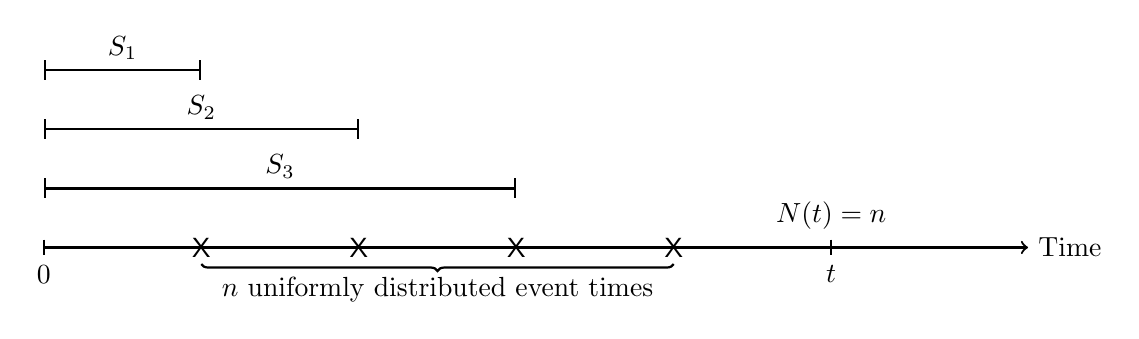
\begin{tikzpicture}[thick]
        \draw[|-|] (0,2.25) -- (2,2.25) node[anchor=south,midway] {$ S_1 $};
        \draw[|-|] (0,1.5) -- (4,1.5) node[anchor=south,midway] {$ S_2 $};
        \draw[|-|] (0,0.75) -- (6,0.75) node[anchor=south,midway] {$ S_3 $};

        \draw[-] (10,0.1) -- (10,-0.1) node[anchor=north] {$t$};
        \node[anchor=south] at (10,0.1) {$ N(t)=n $};

        \node at (2,0) {$ \mathsf{X} $};
        \node at (4,0) {$ \mathsf{X} $};
        \node at (6,0) {$ \mathsf{X} $};
        \node at (8,0) {$ \mathsf{X} $};
        \draw [decoration={brace,mirror,raise=6pt},decorate] (2,0) -- (8,0) node [below=7pt,midway] {$n$ uniformly distributed event times};

        \draw[-] (0,0.1) -- (0,-0.1) node[anchor=north] {$0$};
        \draw[->] (0,0) -- (12.5,0);
        \node[anchor=west] at (12.5,0) {Time};
    \end{tikzpicture}
\end{figure}
\begin{Example}
    \textbf{Example 4.5}. Cars arrive to a toll bridge according to a Poisson process at rate $ \lambda $, where each
    car pays a toll of $\$1$ upon arrival. Calculate the mean and variance of the total amount
        collected by time $t$, \emph{discounted} back to time $0$ where $ \alpha>0 $ is the discount rate per unit time.
        \tcblower{}
        \textbf{Solution}: Let $ N(t) $ count the number of cars arriving to the toll
        bridge by time $ t $, where $ N(t) \sim \POI{\lambda t} $. If
    $ S_i $ denotes the arrival time of the $ i\textsuperscript{th} $
        car of the toll bridge, $ i\in\mathbb{Z}^+ $, then the discounted
        value (i.e., back to time $ 0 $) of $\$1$ paid by the $ i\textsuperscript{th} $
        arrival time is given by
        \[ 1\cdot e^{-\alpha S_i}=e^{-\alpha S_i}, \]
        as demonstrated by the following diagram:
        \begin{center}
            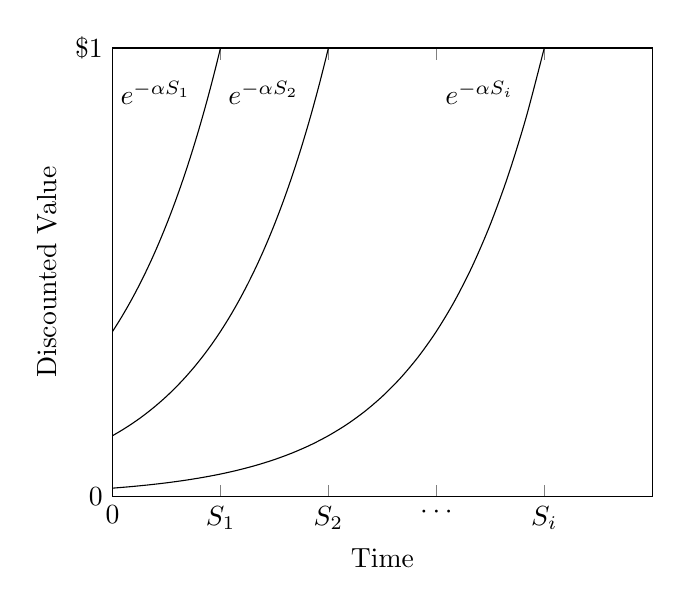
\begin{tikzpicture}
                \begin{axis}[
                        xmin=0, xmax=5,
                        ymin=0, ymax=1,
                        xtick={0,1,2,3,4},
                        xticklabels={$0$,$S_1$,$S_2$,$\cdots$,$S_i$},
                        ytick={0,1},
                        yticklabels={$0$,$\$1$},
                        legend pos=north west,
                        xlabel = Time,
                        ylabel = Discounted Value,
                        extra tick style={tick style={draw=none}},
                    ]
                    \addplot[smooth,domain=0:1]{e^(1*x-1)};
                    \addplot[smooth,domain=0:2]{e^(1*x-2)};
                    \addplot[smooth,domain=0:4]{e^(1*x-4)};
                    \addplot[domain=0:5]{1};
                    \node[] at (axis cs: 0.4,0.9) {$ e^{-\alpha S_1} $};
                    \node[] at (axis cs: 1.4,0.9) {$ e^{-\alpha S_2} $};
                    \node[] at (axis cs: 3.4,0.9) {$ e^{-\alpha S_i} $};
                \end{axis}
            \end{tikzpicture}
        \end{center}
        If $ T $ represents the (discounted) total amount collected by time $ t $,
        then $ T=\sum_{i=1}^{N(t)}e^{-\alpha S_i} $. We wish to find
    $ \E{T} $ and $ \Var{T} $. To find $ \E{T} $, note that
        \begin{align*}
            \E{T}
             & =\E*{\sum_{i=1}^{N(t)}e^{-\alpha S_i}}                                                                                    \\
             & =\sum_{n=1}^{\infty}\E*{\sum_{i=1}^{N(t)}e^{-\alpha S_i}\given N(t)=n}\Prob[\big]{N(t)=n} \text{ since $t=0$ if $N(t)=0$} \\
             & =\sum_{n=1}^{\infty}\E*{\sum_{i=1}^{n}e^{-\alpha S_i}\given N(t)=n}\Prob[\big]{N(t)=n}.
        \end{align*}
        By Theorem 4.7,
        \[ (S_1,S_2,\ldots,S_n)\mid\bigl(N(t)=n\bigr) \sim (Y_{(1)},Y_{(2)},\ldots,Y_{(n)}), \]
        where $ (Y_{(1)},Y_{(2)},\ldots,Y_{(n)}) $ are the $ n $ order statistics from
    $ \Uniform{0,t} $ distribution. As a result,
        \begin{align*}
            \E{T}
             & =\sum_{n=1}^{\infty}\E*{\sum_{i=1}^{n}e^{-\alpha Y_{(i)}}}\Prob[\big]{N(t)=n}                                                                                                                         \\
             & =\sum_{n=1}^{\infty}\E*{\sum_{i=1}^{n}e^{-\alpha Y_{i}}}\Prob[\big]{N(t)=n}\text{ since $ \sum_{i=1}^{n}e^{-\alpha Y_{(i)}}=\sum_{i=1}^{n}e^{-\alpha Y_{i}} $, $ Y_i \sim \Uniform{0,t}\;\forall i $} \\
             & =\sum_{n=1}^{\infty}n\E{e^{-\alpha Y_1}}\Prob[\big]{N(t)=n}.
        \end{align*}
        Clearly,
        \begin{align*}
            \E{e^{-\alpha Y_1}}
             & =\int_{0}^{t}e^{-\alpha y}\frac{1}{t}\odif{y}                       \\
             & =\frac{1}{t}\biggl[\frac{-e^{-\alpha y}}{\alpha}\biggr]_{y=0}^{y=t} \\
             & =\frac{1-e^{-\alpha t}}{\alpha t}.
        \end{align*}
        Therefore,
        \begin{align*}
            \E{T}
             & =\frac{1-e^{-\alpha t}}{\alpha t}\underbrace{\sum_{n=1}^{\infty} n\Prob[\big]{N(t)=n}}_{\E[\big]{N(t)}} \\
             & =\frac{1-e^{-\alpha t}}{\alpha t}\lambda t                                                              \\
             & =\frac{\lambda}{\alpha}(1-e^{-\alpha t}).
        \end{align*}
        To determine $ \Var{T} $, we once again apply Theorem 4.7 to first obtain:
        \begin{align*}
            \Var[\big]{T\given N(t)=n}
             & =\Var[\bigg]{\sum_{i=1}^{n}e^{-\alpha Y_{i}}}                                                                            \\
             & =\Var*{\sum_{i=1}^{n}e^{-\alpha Y_i}}\text{ since $ \sum_{i=1}^{n}e^{-\alpha Y_{(i)}}=\sum_{i=1}^{n}e^{-\alpha Y_{i}} $} \\
             & =\sum_{i=1}^{n}\Var{e^{-\alpha Y_i}}                                                                                     \\
             & =n\Var{e^{-\alpha Y_1}},
        \end{align*}
        due to the independence and iid nature of $ \Set{Y_i}_{i=1}^n $. Note that
    \begin{align*}
        \Var{e^{-\alpha Y_1}}
         & =\E*{(e^{-\alpha Y_1})^2}-\bigl(\E{e^{-\alpha Y_1}}\bigr)^2                  \\
         & =\E*{(e^{-2\alpha Y_1})}-\frac{(1-e^{-\alpha t})^2}{\alpha^2t^2}             \\
         & =\frac{1-e^{-2\alpha t}}{2\alpha t}-\frac{(1-e^{-\alpha t})^2}{\alpha^2t^2},
    \end{align*}
    and so
    \begin{align*}
        \Var[\big]{T\given N(t)}
         & =\Var[\big]{T\given N(t)=n}\Big\vert_{n=N(t)}                                                  \\
         & =N(t)\biggl(\frac{1-e^{-2\alpha t}}{2\alpha t}-\frac{(1-e^{-\alpha t})^2}{\alpha^2t^2}\biggr).
    \end{align*}
    Finally, applying the conditional variance formula, we get
    \begin{align*}
        \Var{T}
         & =\Var[\Big]{\E[\big]{T\given N(t)}}
        +\E[\Big]{\Var[\big]{T\given N(t)}}                                                                                               \\
         & =\Var*{N(t)\cdot \frac{1-e^{-\alpha t}}{\alpha t}}+
        \E*{N(t)\biggl(\frac{1-e^{-2\alpha t}}{2\alpha t}-\frac{(1-e^{-\alpha t})^2}{\alpha^2t^2}\biggr)}                                 \\
         & =\frac{(1-e^{-\alpha t})^2}{\alpha^2t^2}\underbrace{\Var[\big]{N(t)}}_{=\lambda t}
        +\biggl(\frac{1-e^{-2\alpha t}}{2\alpha t}-\frac{(1-e^{-\alpha t})^2}{\alpha^2t^2}\biggr)\underbrace{\E[\big]{N(t)}}_{=\lambda t} \\
         & =\frac{\lambda}{2\alpha}(1-e^{-2\alpha t}).
    \end{align*}
\end{Example}
\begin{Example}
    \textbf{Example 4.6}. Satellites are launched at times according to a Poisson process at rate 3 per
    year. During the past year, it was observed that only two satellites were launched. What is the
    joint probability that the first of these two satellites was launched in the first 5 months of the
    year and the second satellite was launched prior to the last 2 months of the year?
    \tcblower{}
    \textbf{Solution}: Let $ \Set{N(t),t\ge 0} $ be the Poisson process at rate $ \lambda=3 $
    governing satellite launches. We are interested in calculating
    \[ \Prob*{S_1\le \frac{5}{12},S_2\le \frac{5}{6}\given N(1)=2}. \]
    To do so, we use Theorem 4.7 (specifically,~\ref{eq4.12}), to obtain the joint
    conditional pdf of $ (S_1,S_2)\mid\bigl(N(1)=2\bigr) $ as
    \[ g(s_1,s_2)=\frac{2!}{1^2}=2,\; 0<s_1<s_2<1, \]
    which we integrate over the shaded region:
    \begin{center}
        \begin{tikzpicture}
            \begin{axis}[
                    xmin=0, xmax=1.1,
                    ymin=0, ymax=1.1,
                    xtick={0,5/12,1},
                    ytick={0,5/6,1},
                    xticklabels={$0$,$5/12$,$1$},
                    yticklabels={$0$,$5/6$,$1$},
                    legend pos=north west,
                    axis lines=middle,
                    xlabel = $s_1$,
                    ylabel = $s_2$,
                    ymajorgrids=true,
                    xmajorgrids=true,
                    grid style=dashed,
                ]
                \addplot[name path = f,domain=0:1]{x};
                \addplot[name path=null, draw=none]{5/6};
                \addplot[fill=blue,fill opacity=0.05]
                fill between[of=f and null,soft clip={domain=0:5/12},];
            \end{axis}
        \end{tikzpicture}
    \end{center}
    Thus,
    \begin{align*}
        \Prob*{S_1\le \frac{5}{12},S_2\le \frac{5}{6}\given N(1)=2}
         & =\int_{0}^{5/12}\int_{s_1}^{5/6}g(s_1,s_2)\odif{s_2}\odif{s_1}    \\
         & =\int_{0}^{5/12}\int_{s_1}^{5/6}2\odif{s_2}\odif{s_1}             \\
         & =2\int_{0}^{5/12}\biggl(\frac{5}{6}-s_1\biggr)\odif{s_1}          \\
         & =2\biggl[\frac{5}{6}s_1-\frac{s_1^2}{2}\biggr]_{s_1=0}^{s_1=5/12} \\
         & =2\biggl(\frac{25}{72}-\frac{25}{288}\biggr)                      \\
         & =2\times \frac{25}{96}                                            \\
         & =\frac{25}{48}                                                    \\
         & \simeq 0.521.
    \end{align*}
\end{Example}